\chapter{Сценарии и эксперименты}

Эксперименты проводятся в мультиагентной среде multiagent-particle-envs \cite{multiagent-particle-envs} от компании OpenAI.


\section{Эксперименты}

\subsection{Эксперимент на одном мозге}

В алгоритме MADDPG каждый агент имеет набор сетей \textit{критиков}, чтобы иметь собственный механизм оптимизации политики. Тем не менее, два агента в \textit{Simple Reference} полностью симметричны в том смысле, что они оба имеют одинаковое пространство наблюдения, пространство действий и имеют общую глобальную награду. Тем самым агенты формулируют аналогичные оптимальные политики.

Таким образом, каждому агенту можно было бы не создавать свой собственный мозг из сетей критиков, а вместо этого тренировать один мозг для всех агентов. Кроме того, единый мозг MADDPG позволяет агентам общаться на одном «языке», что означает, что они произносят и понимают ориентиры в одних и тех же кодировках.

Так же мы разработали вариант этого алгоритма, можно сказать, что в том случае мы имеем два мозга: один для агентов из одной команды, второй – для агентов из другой команды. Этот вариант мы применили к сценарию \textit{Simple Tag}. Это возможно благодаря тому, что агенты из одной команды в этом сценарии имеют одинаковое пространство наблюдения, пространство действий и имеют общую глобальную награду, но это не так для агентов из разных команд. Поэтому и пришлось использовать отдельный набор сетей для каждой команды.

\subsection{Эксперимент с декомпозированным вознаграждением}

Чтобы обеспечить чёткие сигналы для двух независимых поддействий, мы попробовали реализовать отдельные наборы \textit{актор-критиков} для физического движения и общения.

\begin{figure}[ht!]
    \center
    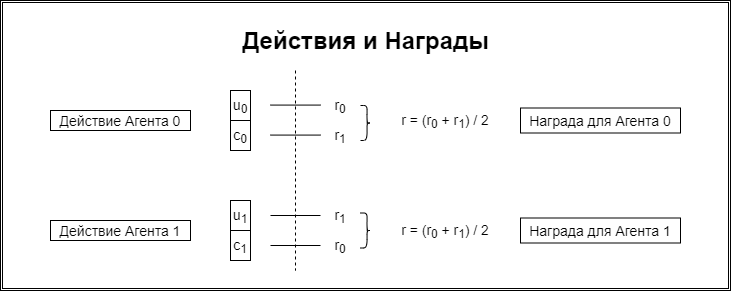
\includegraphics [scale=0.60] {my_folder/images/ch4/actions_and_rewards.png}
    \caption{С левой стороны от пунктирной линии - действие агента, которое представляет собой совокупность физического движения \textit{u} и коммуникационного действия \textit{c}. С правой стороны показано, как награда рассчитывается и назначается для оценки действий. Два агента имеют одинаковую глобальную награду - среднее значение между $r_0$ и $r_1$.}
    \label{fig:action-reward}
\end{figure}

Из \firef{fig:action-reward} видно, что физическое перемещение $u_0$ агента 0 оценивается $r_0$, а высказывание $c_0$ - $r_1$. Окончательное вознаграждение затем раскладывается как кортеж из $r_0$ и $r_1$, т.е. $[r_0; r_1]$, причем каждый элемент соответствует сигналу оценки физического движения и связи соответственно. Точно так же последний набор вознаграждений для агента 1 равен $[r_1; r_0]$.

\begin{figure}[ht!]
    \center
    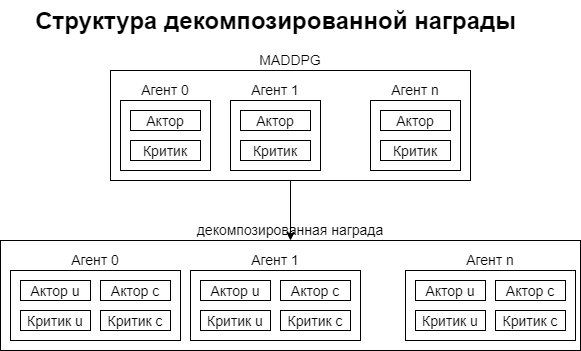
\includegraphics [scale=0.60] {my_folder/images/ch4/decomposed_reward_structure.png}
    \caption{Сетевая структура декомпозированного вознаграждения по сравнению со стандартным MADDPG.}
    \label{fig:decomposed-reward-structure}
\end{figure}

Для физического движения и общения созданы два отдельных набора сетей \textit{актор-критик}, чтобы обеспечить согласованные и точные градиенты для оптимизации двух поддействий, см. \firef{fig:decomposed-reward-structure}. Разложения вознаграждения можно рассматривать как параллельное обучение двух слушателей из \textit{Simple Speaker Listener}. 1 - это агент 0 с коммуникацией $c_0$ в качестве говорящего и агент 1 с физическим движением $u_1$ в качестве слушателя, а 2 - агент 1 с c1 в качестве говорящего и агент 0 с $u_0$ в качестве слушателя, как показано на \firef{fig:action-reward}.

MADDPG с разложенным вознаграждением может быть хорошо приспособлен только к \textit{Simple Reference}, но не может быть обобщён для других игровых сценариев. Поскольку, пространства наблюдений и действий у агентов в этом сценарии симметричны, а главное, каждый агент производит оба вида действия. В большинстве других сценариев это не так. Следовательно, необходимо проводить больше экспериментов с общей глобальной наградой.

\subsection{Эксперимент с обучением по учебной программе}

Обучение по учебной программе применено с целью решения проблемы расходящихся сетей, возникшей в ходе обучения. Примеры обучения организованы в таком порядке, что постепенно вводятся все более сложные концепции.

Варианты учебной программы, на примере сценария Simple Reference:

\begin{itemize}
    \item увеличивать количество ориентиров постепенно. Первый уровень сложности в этой учебной программе с фиксированной целью для обоих агентов, скажем, красным ориентиром в качестве цели. На втором уровне добавляется ещё один ориентир, например зелёный, и цель выбирается случайным образом из двух ориентиров. Последний уровень - это исходная настройка сценария, т. е. рандомизация цели из трех ориентиров. Цель этой учебной программы состоит в том, чтобы агенты учились от простого сценария с меньшим количеством ориентиров к более сложному сценарию со всеми ориентирами;
    \item обучить агента 0 в качестве \textit{говоруна} и агента 1 в качестве \textit{слушателя} на первом этапе, а на следующем этапе обучить двух агентов в качестве \textit{говорунов} и \textit{слушателей} в исходном игровом сценарии;
    \item предоставить агентам заранее определенные коммуникационные действия для трёх цветов, скажем, [1; 0; 0] для красного, [0; 1; 0] для зелёного и [0; 0; 1] для синего. Таким образом, первая фаза состоит в том, чтобы изучить физическое движение, чтобы правильно двигаться. Затем, одному из агентов больше не предоставляются предопределённые коммуникационные действия, но взамен предоставляется связь с другим агентом (показываются его коммуникационные действия). Ожидается, что другому агенту будет легче научиться правильно общаться. Наконец, мы возвращаемся к исходным игровым настройкам для двух агентов, когда изучаются как физическое движение, так и общение.
\end{itemize} % TODO: каждый пункт - новое предложение?


\section{Метрики измерения консистентности коммуникационных действий}

Обучение модели можно ориентировочно оценивать на глаз при рендеринге физического движения, но можно и создать метрику и строить по ней графики. Выбранная метрика для коммуникационных действий заключается в том, что агент должен однозначно интерпретировать комунникационные действия и выбирать соответствующие им цвета цели.

Методика, используемая для измерения сходимости коммуникации, заключается в том, что мы создаем матрицу которая сопоставляет интерпретацию агента и текущий цвет цели. Допустим, строки – это цвета целей, а коммуникационные действия представлены в one hot encoded строках (строки, в которых максимальное значение в векторе действия представляется в виде 1, а остальные – 0). Тогда после нормализации матрицы, если обучение сходится, она должна выглядеть примерно так:

\begin{equation*}
    \begin{bmatrix}
        1 & 0 & 0 \\
        0 & 1 & 0 \\
        0 & 0 & 1
    \end{bmatrix}
\end{equation*}

или

\begin{equation*}
    \begin{bmatrix}
        1 & 0 & 0 \\
        0 & 0 & 1 \\
        0 & 1 & 0
    \end{bmatrix}
\end{equation*}

и т. д.

Не важно, как агенты интерпретируют цвета, \textit{детерминант} этой матрицы, в конце концов, стремиться к 1 или -1. Мы в своих экспериментах использовали этот способ.

Ещё один способ измерения заключается в том, чтобы смотреть, какое действие коммуникации выбрал говорун, при наблюдении определённого цвета и проверять, совпадает ли оно с тем, что было выбрано в прошлый раз с тем же наблюдением. График с результатом должен приблизиться к $100\%$ после схождения.

\section{Сценарии}

\subsection{Сценарий 1. Simple Speaker Listener}  \label{exp-ssl}

Сценарий Simple Speaker Listener воспроизводится и тестируется с использованием алгоритма MADDPG \cite{lowe2017multiagent}.

Сценарий упоминается в разделе \hyperref[intro:ssl]{Вводная глава: Сценарий 1. Simple Speaker Listener}. В этом сценарии два агента имеют разные пространства действий и наблюдений. Наблюдение говоруна $o_s$~--- это цвет цели, обозначенный 3- канальным вектором $d \in \mathbb{R}^3$. Наблюдение слушателя $o_l$ – это вектор конкатенации его собственной скорости $\upsilon \in \mathbb{R}^2$ его расстояния до трёх ориентиров $p = [p_1, p_2, p_3], p_i \in \mathbb{R}$ и сигнал, произнесённый говоруном на предыдущем временном шаге:

\begin{equation}
    \begin{multlined}
        o_s = [d], \\
        o_l = \begin{bmatrix}
                  \upsilon \\ p \\ c
        \end{bmatrix}.
    \end{multlined}
\end{equation}

Коммуникационное действие говоруна обозначается «one-hot encoding» вектором ${[1; 0; 0]}$, или ${[0; 1; 0]}$, или ${[0; 0; 1]}$ для обозначения трёх ориентиров соответственно.
Физическое действие u слушателя~--- это 5-канальный вектор, каждый из которых представляет одно направление движения (вверх, вниз, влево, вправо или без движения). Наблюдения и действия говоруна и слушателя и их взаимосвязь показаны на рисунке \firef{fig:ch4-ssl}.

\begin{figure}[ht!]
    \center
    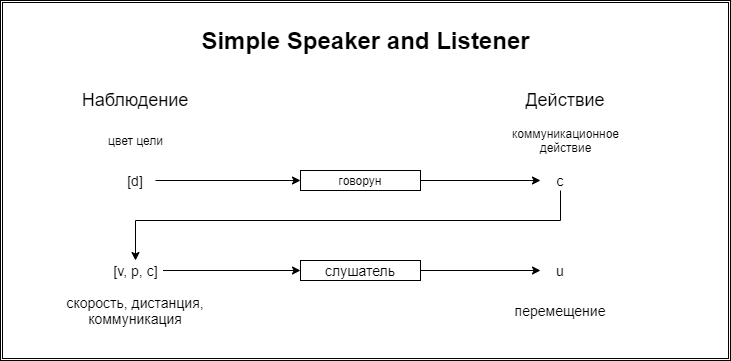
\includegraphics [scale=0.60] {my_folder/images/ch4/simple_speaker_listener.png}
    \caption{Говорун наблюдает цвет целевого ориентира d и издаёт коммуникационое действие, которое будет получено слушателем. Слушатель производит физическое движение}
    \label{fig:ch4-ssl}
\end{figure}

Два агента имеют общую награду r, которая является отрицательным евклидовым расстоянием между слушателем и его целью. Проблема, которую необходимо решить в этом сценарии, заключается в поиске оптимальных политик для говоруна и слушателя, чтобы максимизировать ожидаемую награду, то есть найти $\max_{\pi}R(\pi)$, где

\begin{equation}
    \begin{multlined}
        R(\pi) = \mathbb{E}[\sum_{t=0}^{T}r(s_t, a_t)].
    \end{multlined}
\end{equation}

Во время обучения говорун учится различать три ориентира и передавать целевой ориентир слушателю. И слушатель должен изучить закодированные высказывания говоруна и перейти к правильной цели.

Архитектура актор-сети говоруна аналогична архитектуре слушателя, каждый из которых содержит два полносвязанных слоя с 64 нейронами и использует функцию активации relu. Однако их выходные слои различаются с точки зрения количества единиц. Сети критиков имеют структуру, аналогичную сетям акторов, за исключением того, что они выдают скалярное Q-значение.

На этом сценарии было произведено измерение консистентности коммуникационных действий для алгоритмов DDPG и MADDPG.

\subsection{Сценарий 2. Simple Reference} \label{exp-sr}

Simple Reference~--- это более сложный сценарий, который расширяет Simple Speaker Listener.

Проблема, которую необходимо решить в этом сценарии, была изложена в разделе \hyperref[intro-sr]{Вводная глава: Сценарий 2. Simple Reference}. На \firef{fig-intro-sr} показан сценарий игры и поведение агентов при использовании оптимальных политик. В этом сценарии оба агента одновременно выступают и слушателями, и говорунами, что означает, что они оба выполняют как физические, так и коммуникационные действия. Высказывание каждого агента на одном шаге наблюдается другим агентом на следующем шаге, как показано на \firef{fig:exp-sr}.

Каждый агент наблюдает скорость, расстояние до ориентиров, цвет цели другого агента и высказывание другого агента. Действие каждого агента состоит из двух поддействий: физического движения $u$ и коммуникационного действия $c$.

Наблюдение и действие:

\begin{equation}
    \begin{multlined}
        o_i = \begin{bmatrix}
                  \upsilon \\ p \\ d \\ c
        \end{bmatrix}, \\
        a_i = \begin{bmatrix}
                  u \\ c
        \end{bmatrix}.
    \end{multlined}
\end{equation}


Это показано на \firef{fig:exp-sr}.

Наградой каждого агента является среднее значение отрицательных евклидовых расстояний от агентов до их целей. Таким образом, оцениваются как физические, так и коммуникационные действия агентов. Предположим, что $r_0$~--- это отрицательное евклидово расстояние от агента 0 до его цели, а $r_1$~--- это расстояние от агента 1 до его цели. Окончательная награда для каждого агента:

\begin{equation}
    \begin{multlined}
        r = \frac{r_0 + r_1}{2}.
    \end{multlined}
\end{equation}

Награда $r_0$ используется для оценки физического движения $u_0$ агента 0 и коммуникационного действия $c_1$ агента 1. То же относится и к $r_1$ - он используется для оценки физического движения $u_1$ агента 1 и высказывания $c_0$ агента 0. Это показано на \firef{fig:exp-sr}.

Архитектура нейронных сетей актора-критика двух агентов в этом сценарии аналогична архитектуре в предыдущем сценарии.

\begin{figure}[ht!]
    \center
    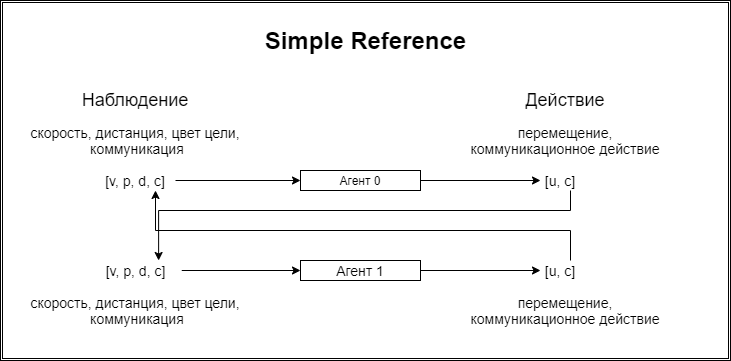
\includegraphics [scale=0.60] {my_folder/images/ch4/simple_reference.png}
    \caption{Каждый агент наблюдает целевой ориентир другого и производит коммуникационное действие, которое будет получено другим агентом на следующем шаге}
    \label{fig:exp-sr}
\end{figure}

В этом сценарии был поставлен эксперимент с декомпозированным вознаграждением, а также эксперимент с общим мозгом

Так же на этом сценарии производилось измерение консистентности коммуникационных действий.

\subsection{Сценарий 3. Simple World Communication} \label{exp-swc}

Кратко этот сценарий был описан в разделе \hyperref[intro-swc]{Вводная глава: Сценарий 3. Simple World Communication}. На \firef{fig:swc} показан сценарий игры и поведение агентов при использовании оптимальных политик. В этом сценарии лидер выступает говоруном, остальные преследователи – слушателями. И те, и другие перемещаются в погоне за хорошими агентами. Лидер выступает говоруном, а преследователи~--- слушателями. Высказывание лидера на одном шаге наблюдается другими преследователями на следующем шаге, как показано на \firef{fig:exp-swc}.

Хорошие агенты просто наблюдают еду и преследователей и перемещаются.

Под едой подразумевается объект, при приближении к которому, хорошие агенты получают награду

\begin{figure}[ht!]
    \center
    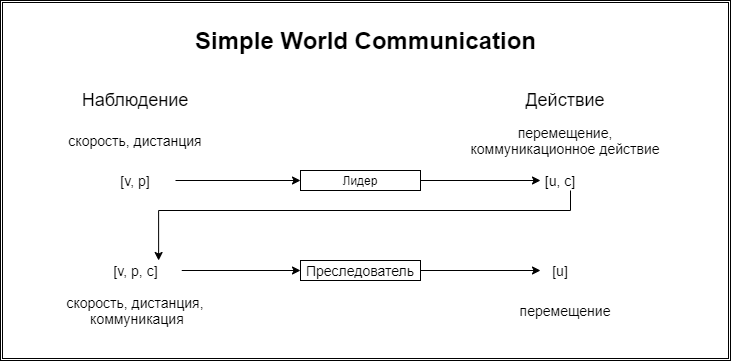
\includegraphics [scale=0.60] {my_folder/images/ch4/simple_world_communication.png}
    \caption{Лидер видит то, чего, возможно, не видят другие преследователи, и производит коммуникационное действие, которое будет получено преследователями на следующем шаге}
    \label{fig:exp-swc}
\end{figure}

Каждый преследователь наблюдает скорость $\upsilon \in \mathbb{R}^2$, расстояние до жертв $p = [p_1, p_2, p_3], p_i \in \mathbb{R}$, и высказывание лидера. Лидер наблюдает то же самое, кроме высказывания. Действие лидера состоит из двух поддействий: физического движения $u$ и коммуникационного действия $c$. Действие преследователя – только из физического движения $u$.
Наблюдение и действие лидера:

\begin{equation}
    \begin{multlined}
        o_i = \begin{bmatrix}
                  \upsilon \\ p
        \end{bmatrix}, \\
        a_i = \begin{bmatrix}
                  u \\ c
        \end{bmatrix}.
    \end{multlined}
\end{equation}

Наблюдение и действие преследователя:

\begin{equation}
    \begin{multlined}
        o_i = \begin{bmatrix}
                  \upsilon \\ p \\ c
        \end{bmatrix}, \\
        a_i = \begin{bmatrix}
                  u
        \end{bmatrix}.
    \end{multlined}
\end{equation}

Это показано на рисунке \firef{fig:exp-swc}.

Наградой каждого преследователя является отрицательное евклидово расстояние до ближайшего агента.

Во время обучения лидер учится, как закодировать положение жертвы, чтобы передать его преследователю. И преследователь должен изучить закодированные высказывания лидера и двигаться к жертве.

Архитектура нейронных сетей в этом сценарии аналогична архитектуре в предыдущем сценарии.

На этом сценарии производилось измерение консистентности коммуникационных действий.

\subsection{Сценарий 4: Simple Tag} \label{exp-st}

Кратко этот сценарий был описан в разделе \hyperref[intro-st]{Вводная глава: Сценарий 4. Simple Tag}. На \firef{fig:st} показан сценарий игры и поведение агентов при использовании оптимальных политик. В этом сценарии нет общения между агентами, но пространства наблюдения и действий всех преследователей совпадают, это позволяет применить к нему метод обучения с одним мозгом. В этом сценарии все агенты наблюдают друг друга и перемещаются по игровому полю.

Каждый преследователь наблюдает скорость $\upsilon \in \mathbb{R}^2$, расстояние до жертв ${p = [p_1, p_2, p_3], p_i \in \mathbb{R}}$.

Наблюдение и действие:

\begin{equation}
    \begin{multlined}
        o_i = \begin{bmatrix}
                  \upsilon \\ p
        \end{bmatrix}, \\
        a_i = \begin{bmatrix}
                  u
        \end{bmatrix}.
    \end{multlined}
\end{equation}

Наградой каждого преследователя является отрицательное евклидово расстояние до ближайшего агента.

Во время обучения преследователи учатся догонять жертву, а жертва – убегать.

Архитектура нейронных сетей в этом сценарии аналогична архитектуре в предыдущем сценарии.

На этом сценарии ставился эксперимент с одним мозгом.


\section{Сетевая архитектура} \label{network-architecture}

В таблице \taref{tab-algs-application} показана примененимость различных сетевых архитектур к различным игровым сценариям.

\begin{table}[t!]
    \centering\small
    \caption{Подходящие сетевые архитектуры для разных игровых сценариев}
    \label{tab-algs-application}
    \begin{tabular}{|l|l|l|l|l|l|}
        \hline
        & MADDPG & MADDPG с одним мозгом & Декомпозированная награда \\
        \hline
        Speaker Listener    & v      & ---                   & ---                       \\ \hline
        Simple Reference    & v      & v                     & v                         \\ \hline
        World Communication & v      & ---                   & v                         \\ \hline
        Simple Tag          & v      & v                     & ---                       \\ \hline
    \end{tabular}
    \normalsize% возвращаем шрифт к нормальному
\end{table}

Такие сценарии как Simple Speaker Listener с двумя агентами, разделяющими глобальное вознаграждение, но обладающими разными наблюдениями и пространствами действий, могут использовать только стандартный MADDPG. Поскольку агенты функционируют по-разному, им необходимо искать различные оптимальные политики для своих ролей в игре.

Такие сценарии как Simple Reference, где два агента совместно получают глобальное вознаграждение, имеют одно и то же пространство действий и пространство наблюдений, могут работать со стандартным MADDPG, а также эти сценарии могут использовать общий мозг или декомпозированную награду.

Наиболее эффективной архитектурой являются использование сети с общим мозгом, поскольку при этом обучается меньшее количество сетей. Это значительно повышает эффективность обучения игровых сценариев, которые можно адаптировать к сетям с общим мозгом.

В сценарии Simple Tag агенты из одной команды также имеют одинаковые пространства наблюдений и действий. Здесь был применён отдельный набор акторов-критиков для преследователей и отдельный - для жертв. Общение в этом сценарии отсутствует, поэтому декомпозированная награда здесь не применима. Этот сценарий был выбран для сравнения стандартного MADDPG и MADDPG с одним мозгом.

В экспериментах со сценариями, в которых агенты общаются между собой (см. \taref{tab-communicational-scenarious}), производилось измерение консистентности коммуникационных действий.

\begin{table}[t!]
    \centering\small
    \caption{Наличие действий общения в сценариях}
    \label{tab-communicational-scenarious}
    \begin{tabular}{|l|l|l|l|l|l|}
        \hline
        & Предполагает общение агентов \\
        \hline
        Speaker Listener    & v                            \\
        \hline
        Simple Reference    & v                            \\
        \hline
        World Communication & v                            \\
        \hline
        Simple Tag          & ---                          \\
        \hline
    \end{tabular}
    \normalsize% возвращаем шрифт к нормальному
\end{table}

Сценарии, в которых одни и те же агенты и перемещаются и говорят, подходят для применения декомпозированой награды. Simple Listener не подходит, т.к. один агент только перемещается, а другой только говорит, а в Simple Tag нет действий общения.

Таким образом, для ответа на \hyperref[intro-questions]{вопросы исследования} ставились эксперименты, показывающие общение агентов между собой, а также эксперименты, показывающие эффективность некоторых модификаций алгоритма, направленных на ускорение обучения. Исходя из этого и выбирались сценарии для экспериментов данной работы.

